
\subsection{Создание механизма 
сглаживания и фильтрации данных акселерометра и 
гироскопа (Агаев Фархат)}
Моей главной задачей являлось написть фильтр, 
который сможет сгладить данные и избавиться от шума.
Чтобы применить правильный фильтр нужно понять природу шума, 
почему датчик акселерометра искажает данные.
\subsubsection{Природа шума}
Для начала нарисуем график по трем осям (начнем с акселерометра), 
когда телефон лежит на столе. Посмотрим есть какие-либо перепады

\begin{figure}[H]
    \begin{center}
        \begin{tabular}{cc}
            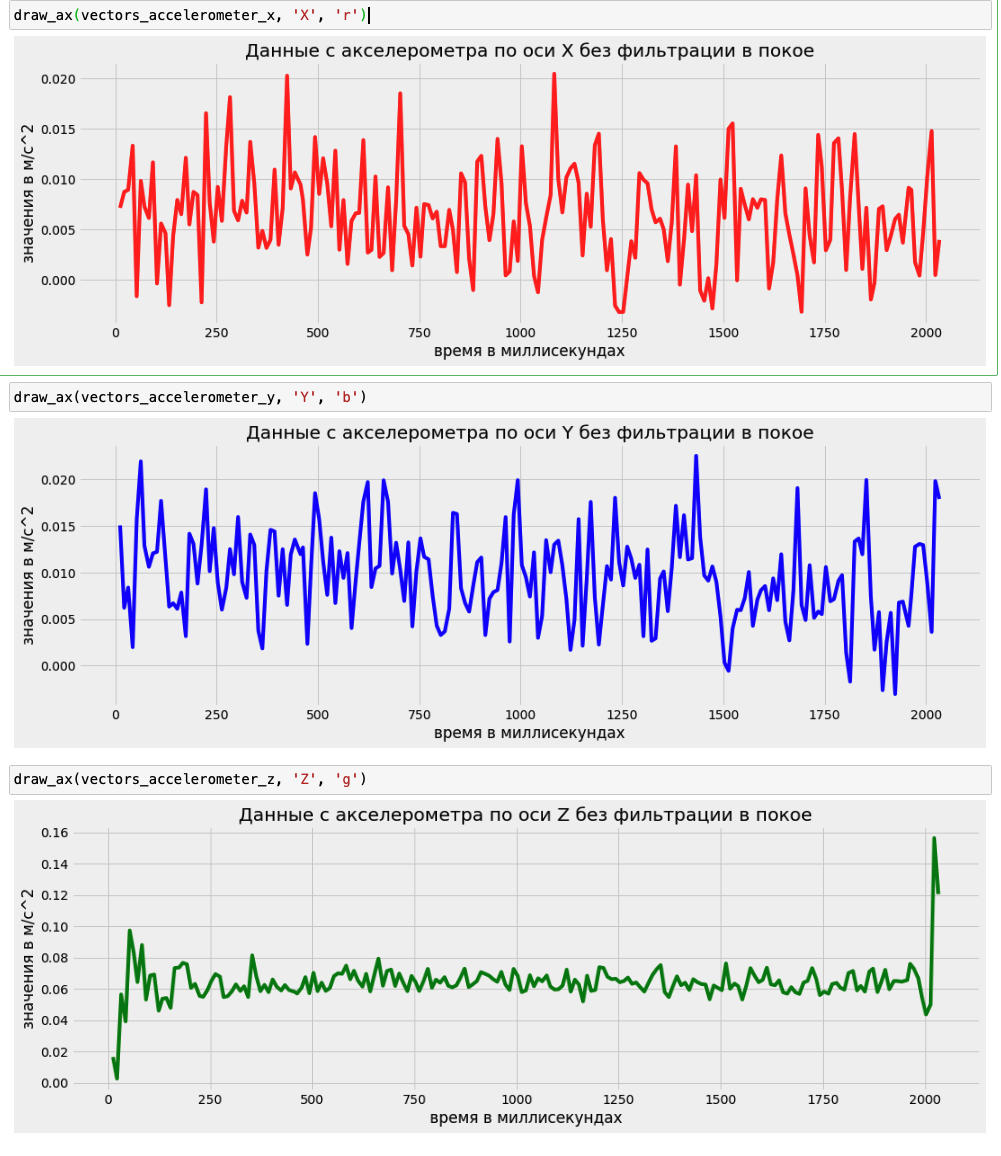
\includegraphics[width=0.75\textwidth]{farim/shakeee} & 
        \end{tabular}
    \end{center}
\end{figure}

На графике хорошо видно, что есть высокочастотные сигналы, 
когда телефон просто лежит на столе от -0.025  до 0.025 $\text{м}/\text{с}^2$. То есть
погрешность уже состовляет более двух процентов. 

\begin{figure}[H]
    \begin{center}
        \begin{tabular}{cc}
            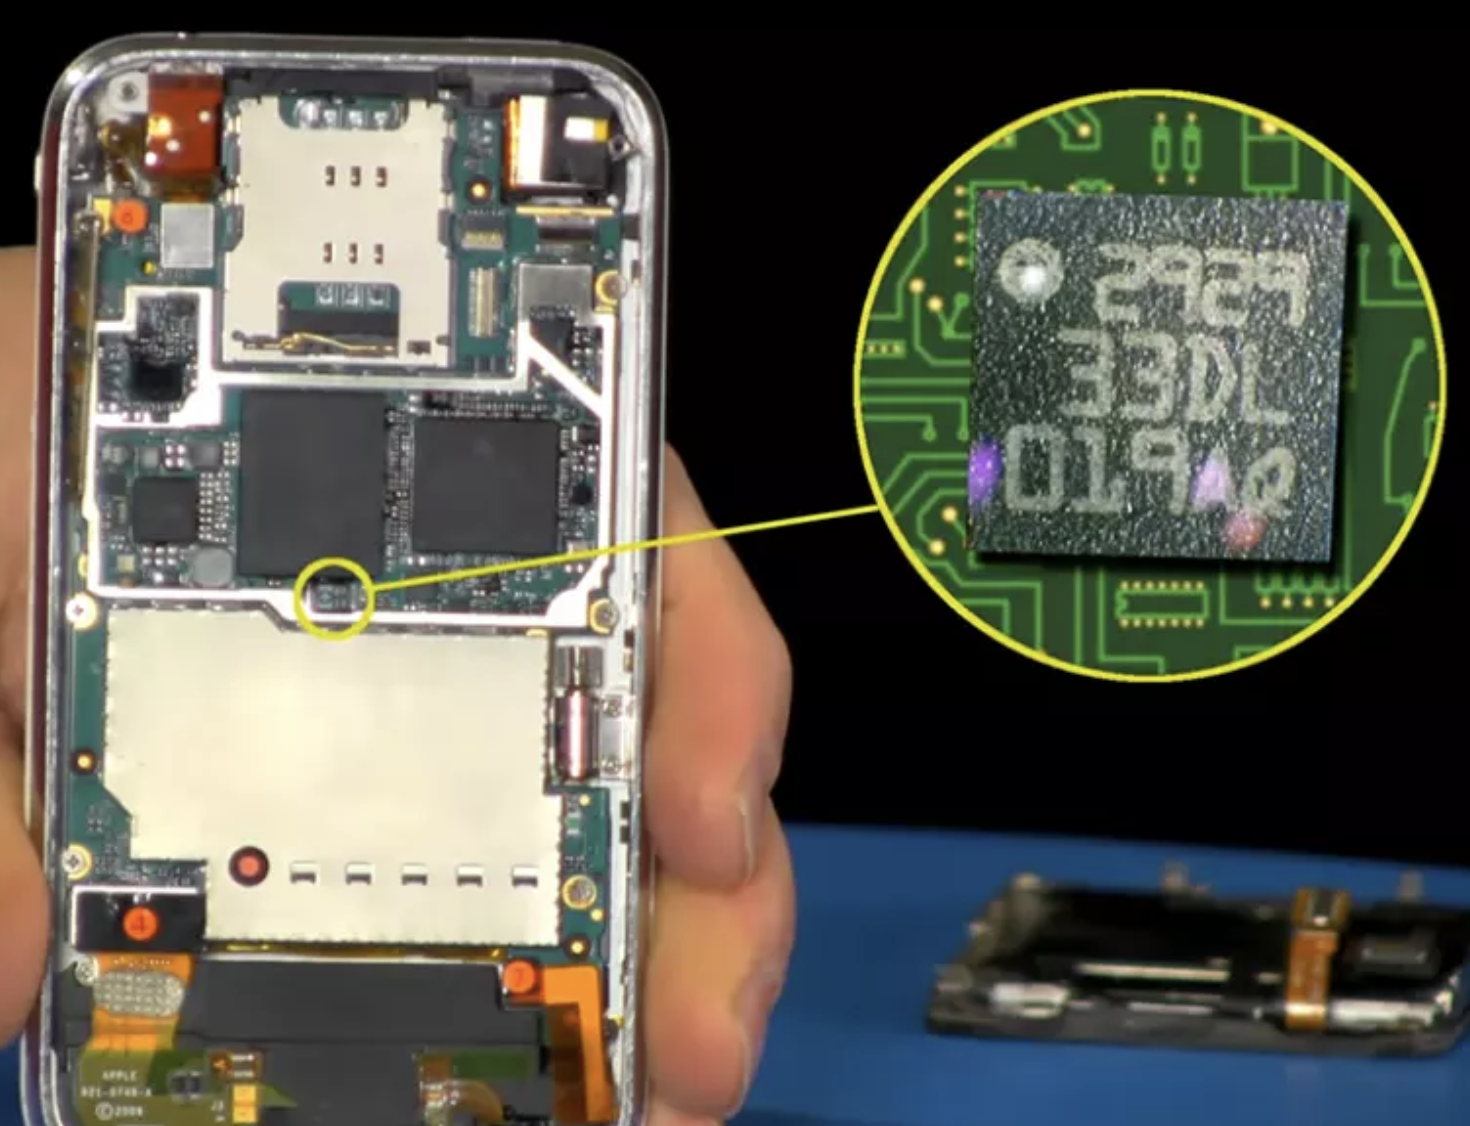
\includegraphics[width=0.5\textwidth]{farim/im2} & 
            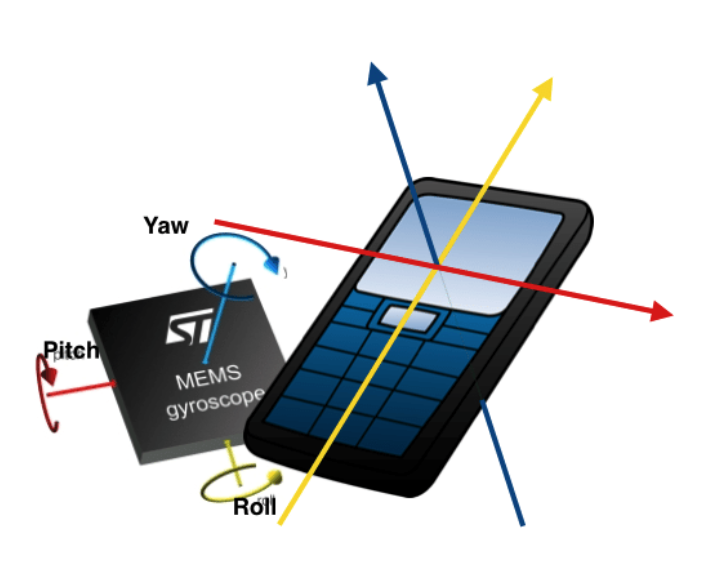
\includegraphics[width=0.5\textwidth]{farim/im3}
        \end{tabular}
    \end{center}
    \caption{изображение датчика акселерометра и гироскопа.}
\end{figure}
Также на величину выходного сигнала акселерометра в основном влияют:
\begin{enumerate}
    \item температура окружающей среды и места крепления акселерометра (температурные погрешности);
    \item внешние магнитные поля (погрешности от магнитного поля);
    \item вибрация и угловые колебания основания (вибрационные погрешности);
    \item частотные характеристики акселерометра (частотные погрешности);
    \item гистерезис показаний (одна из составляющих нелинейности).
\end{enumerate}



\newpage
Теперь взглянум на график разных жестов 
\begin{figure}[H]
    \begin{center}
        \begin{tabular}{cc}
            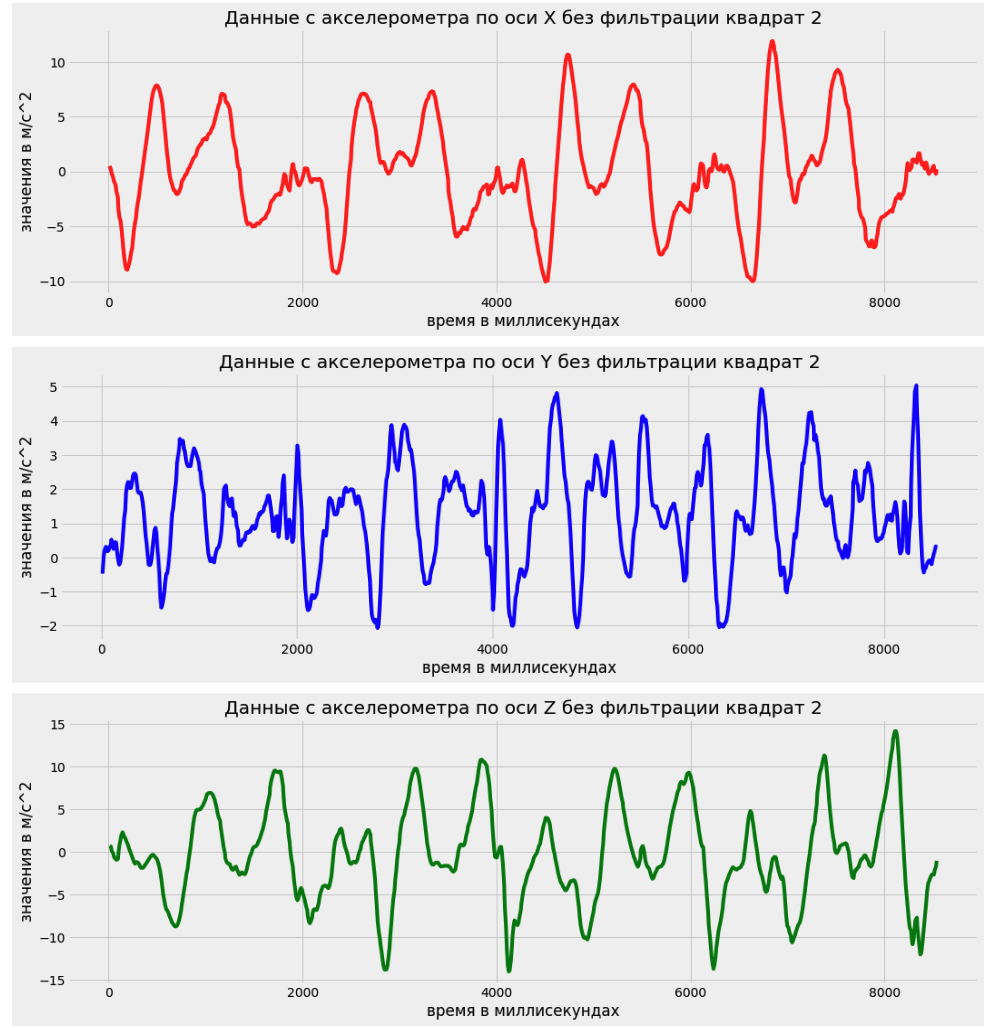
\includegraphics[width=1\textwidth]{farim/sq} & 
        \end{tabular}
    \end{center}
\end{figure}

Хорошо видны всплески и  резкие искажения, их нужно будет сгладить

\begin{figure}[H]
    \begin{center}
        \begin{tabular}{cc}
            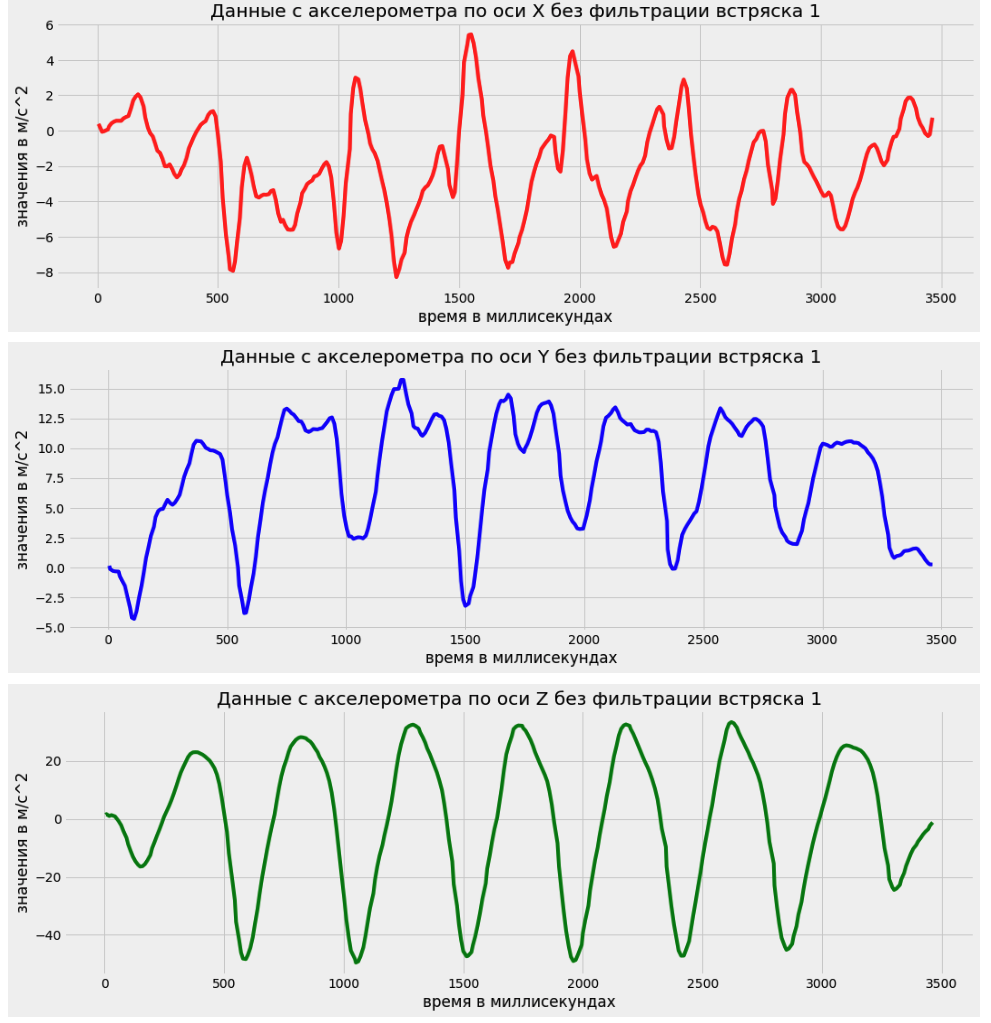
\includegraphics[width=1\textwidth]{farim/shakeeee.png} & 
        \end{tabular}
    \end{center}
\end{figure}

Когда происходит встряска график получается более гладкий особенно по оси Z.
Теперь рассмотрим жест круг, для больше точности и понимания
Посмотрим графики несколько кругов, полученных при разной скорости их реализации.
Круги будут идти с возрастающей скоростью.
Также рассмотрим круги с разными радиусами, попробуем понять, насколько сильно будут портиться данные.

\begin{figure}[H]
    \begin{center}
        \begin{tabular}{cc}
            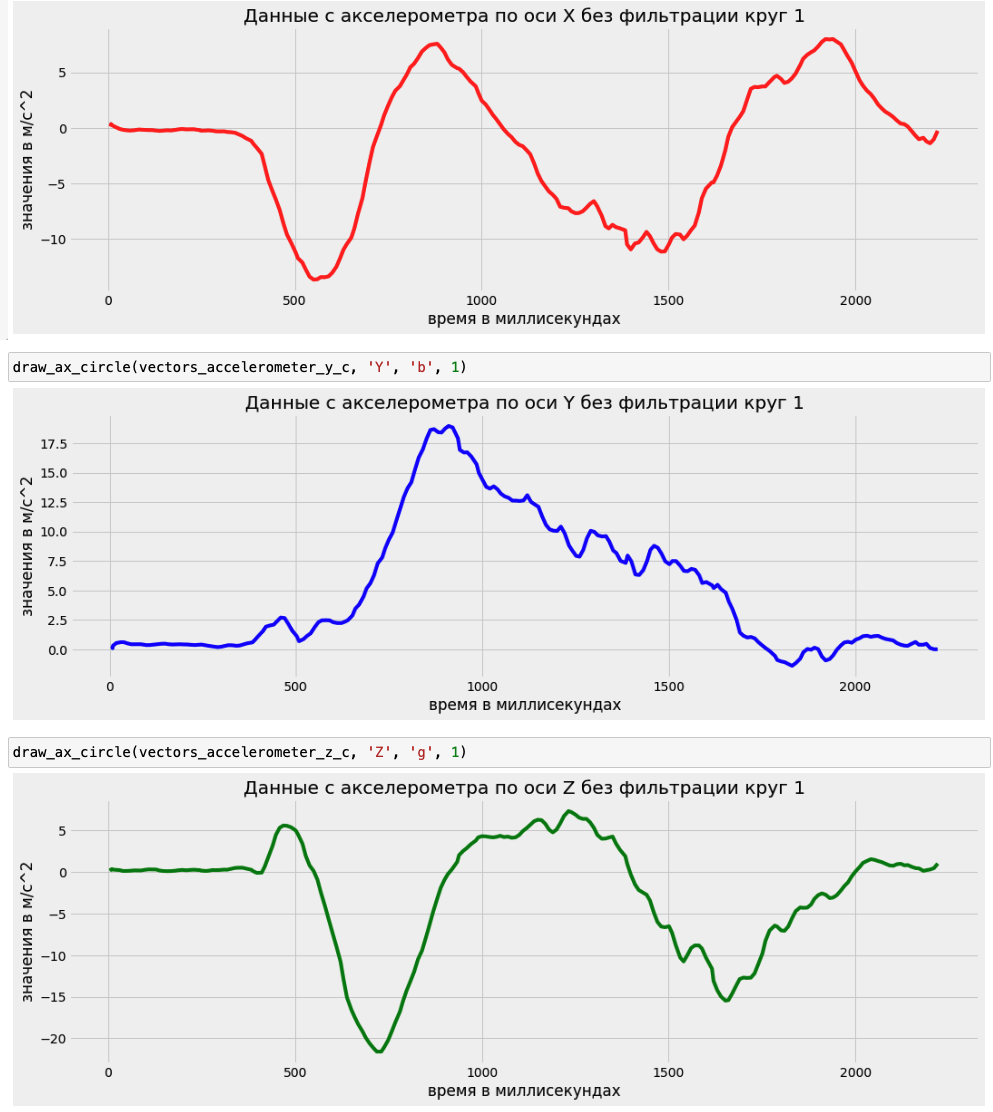
\includegraphics[width=1\textwidth]{farim/cirx} & 
        \end{tabular}
    \end{center}
\end{figure}


\begin{figure}[H]
    \begin{center}
        \begin{tabular}{cc}
            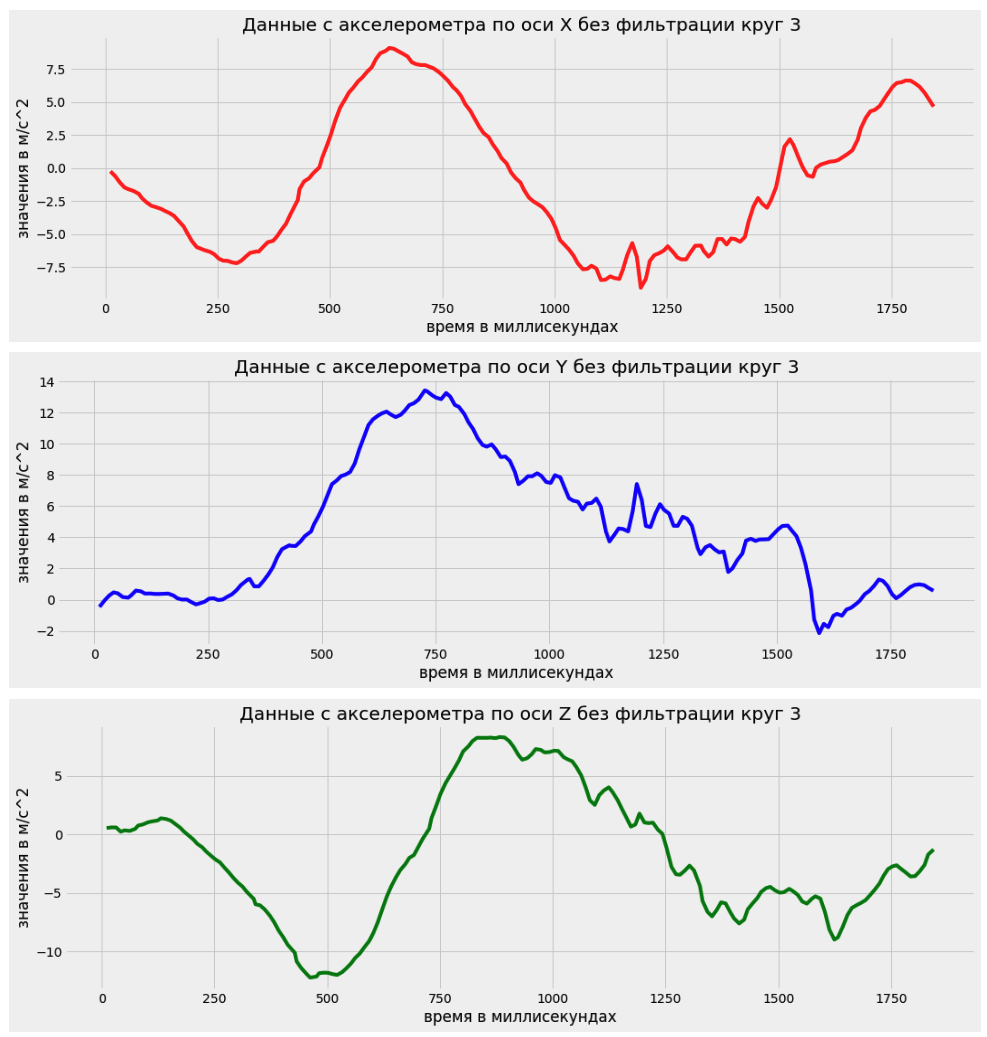
\includegraphics[width=1\textwidth]{farim/im4.png} & 
        \end{tabular}
    \end{center}
\end{figure}


\newpage
\begin{figure}[H]
    \begin{center}
        \begin{tabular}{cc}
            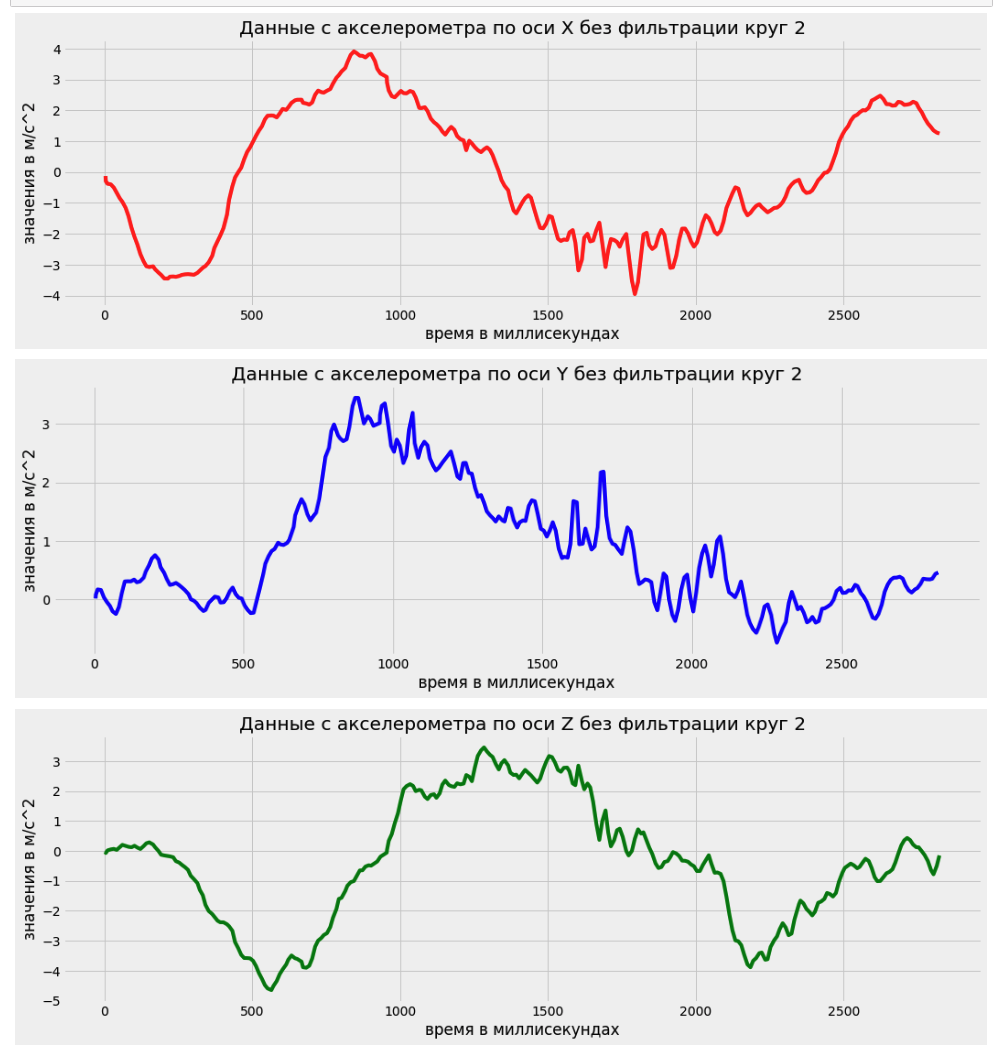
\includegraphics[width=1\textwidth]{farim/im5.png} & 
        \end{tabular}
    \end{center}
\end{figure}


\begin{figure}[H]
    \begin{center}
        \begin{tabular}{cc}
            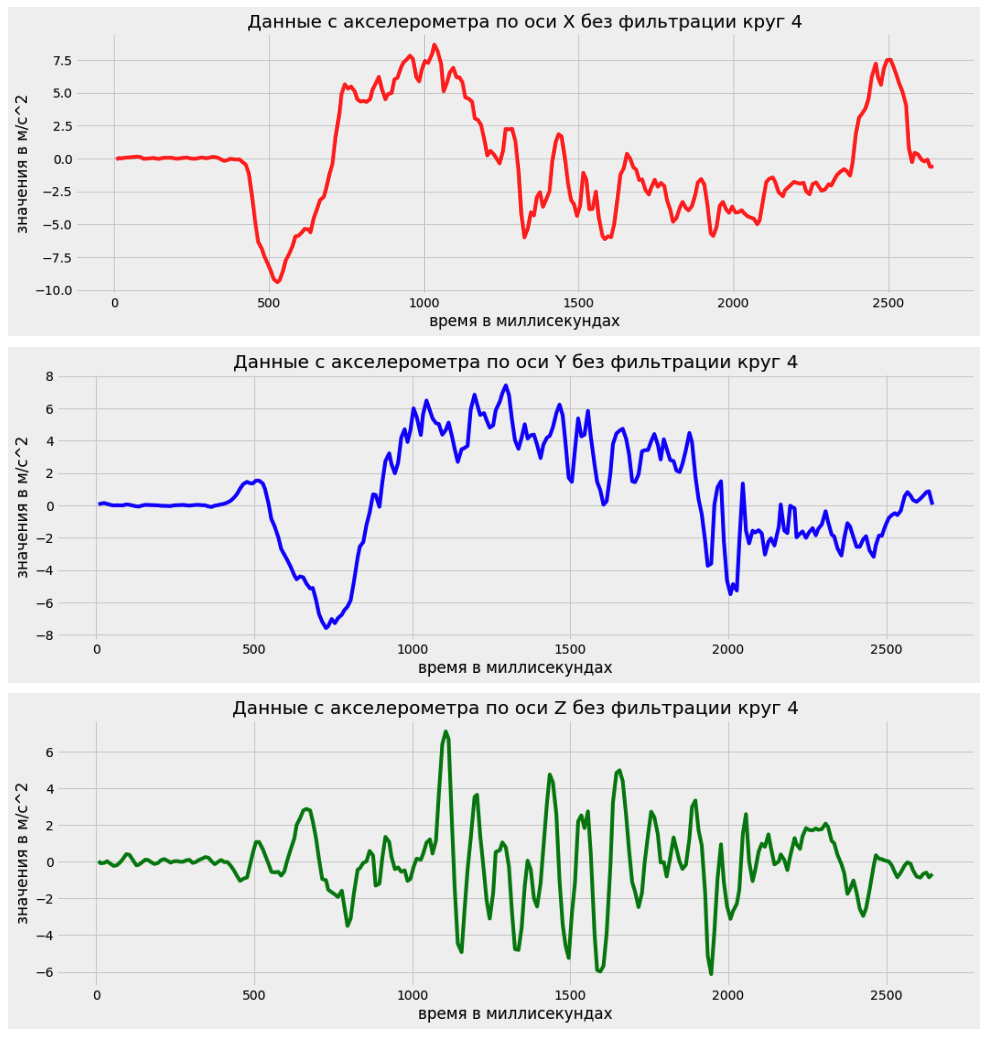
\includegraphics[width=1\textwidth]{farim/im6.png} & 
        \end{tabular}
    \end{center}
\end{figure}


\begin{figure}[H]
    \begin{center}
        \begin{tabular}{cc}
            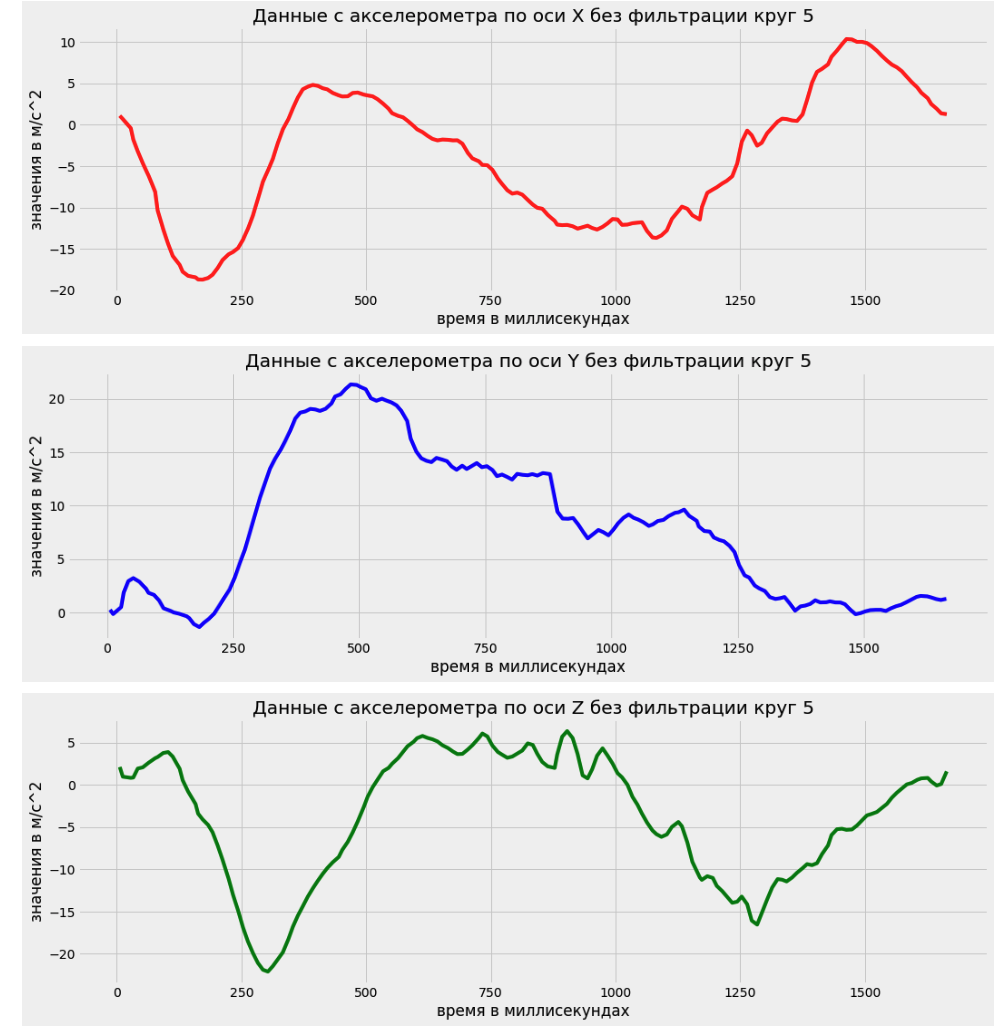
\includegraphics[width=1\textwidth]{farim/im7.png} & 
        \end{tabular}
    \end{center}
\end{figure}
Как мы можем заметить главная проблема - высокие частоты и очень резкие переходы в этом случае.
для нас идеально подойдет фильтр нижних частот.






\newpage
\subsubsection{Принцип работы}

Это фильтр, который пропускает сигналы с 
частотой ниже выбранной частоты среза и 
ослабляет сигналы с частотами выше, чем частота
среза.
В нашем случае я подобрал частоту среза равную  0.6 Гц (Опытным путем построения графиков так, чтобы 
не сильно уходить от данных полученных непосредственно от датчика и максимально хорошо сгладить данные)
Фильтр реализован с помошью питоновских библиотек scipy, numpy (код есть на гитхабе) 
Воспользуемся фильтром и посмотрим результат работы
\begin{figure}[H]
    \begin{center}
        \begin{tabular}{cc}
            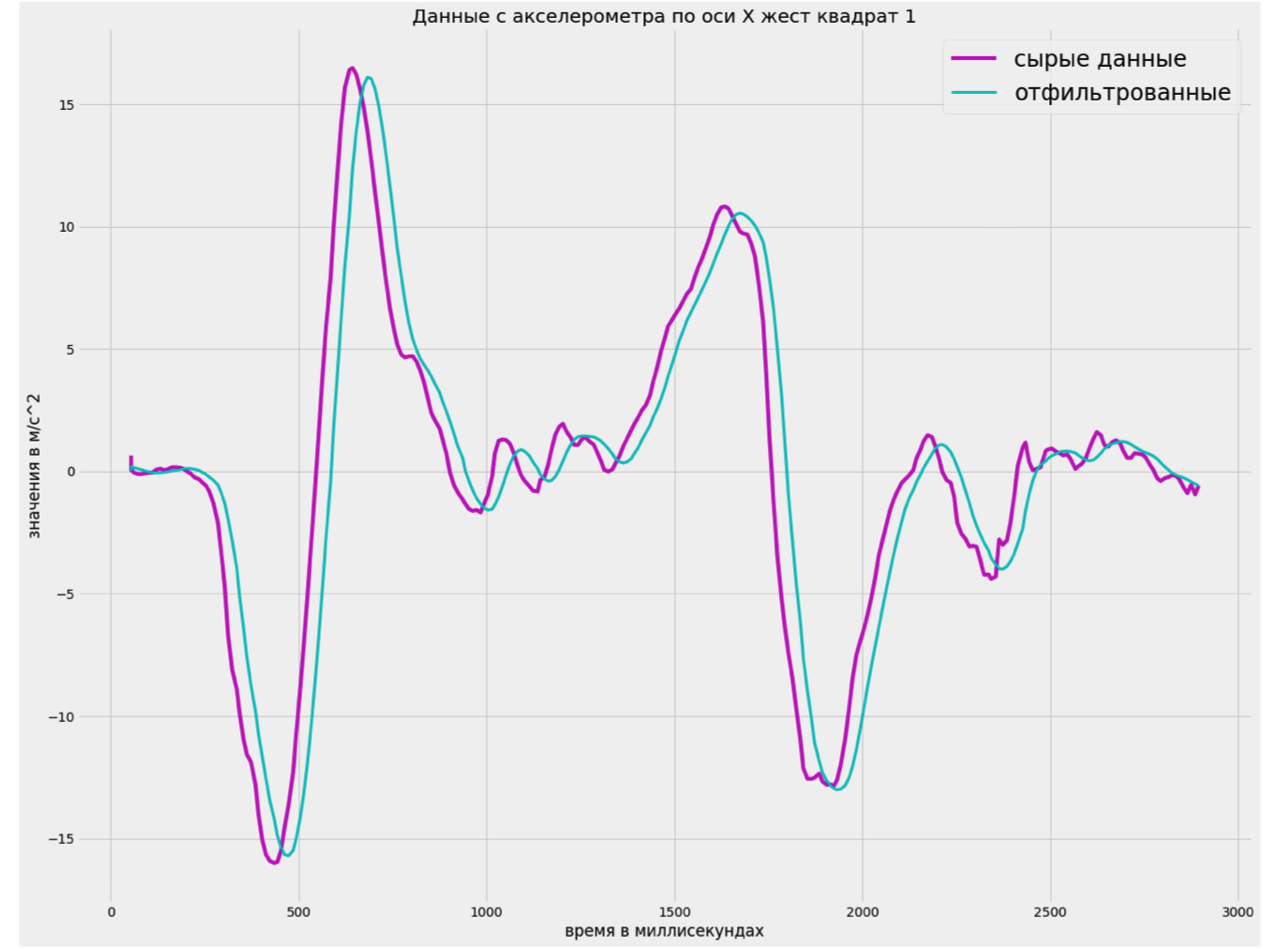
\includegraphics[width=0.75\textwidth]{farim/squares} & 
        \end{tabular}
    \end{center}
\end{figure}
\begin{figure}[H]
    \begin{center}
        \begin{tabular}{cc}
            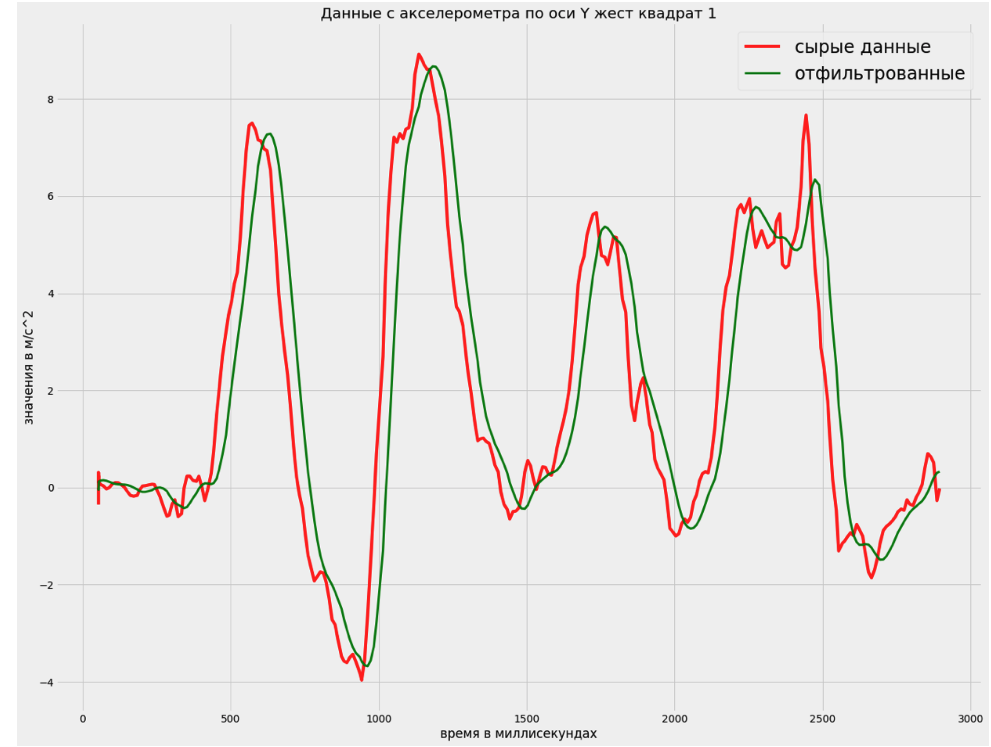
\includegraphics[width=0.75\textwidth]{farim/sqxres} & 
        \end{tabular}
    \end{center}
\end{figure}

\begin{figure}[H]
    \begin{center}
        \begin{tabular}{cc}
            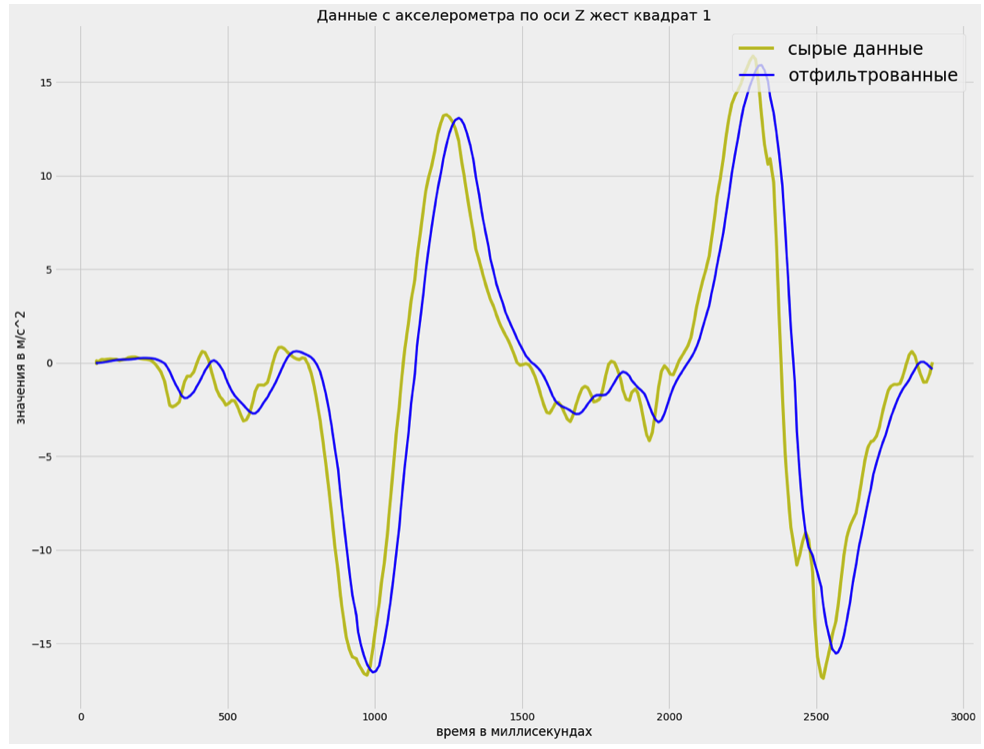
\includegraphics[width=0.75\textwidth]{farim/sqzres} & 
        \end{tabular}
    \end{center}
\end{figure}

\begin{figure}[H]
    \begin{center}
        \begin{tabular}{cc}
            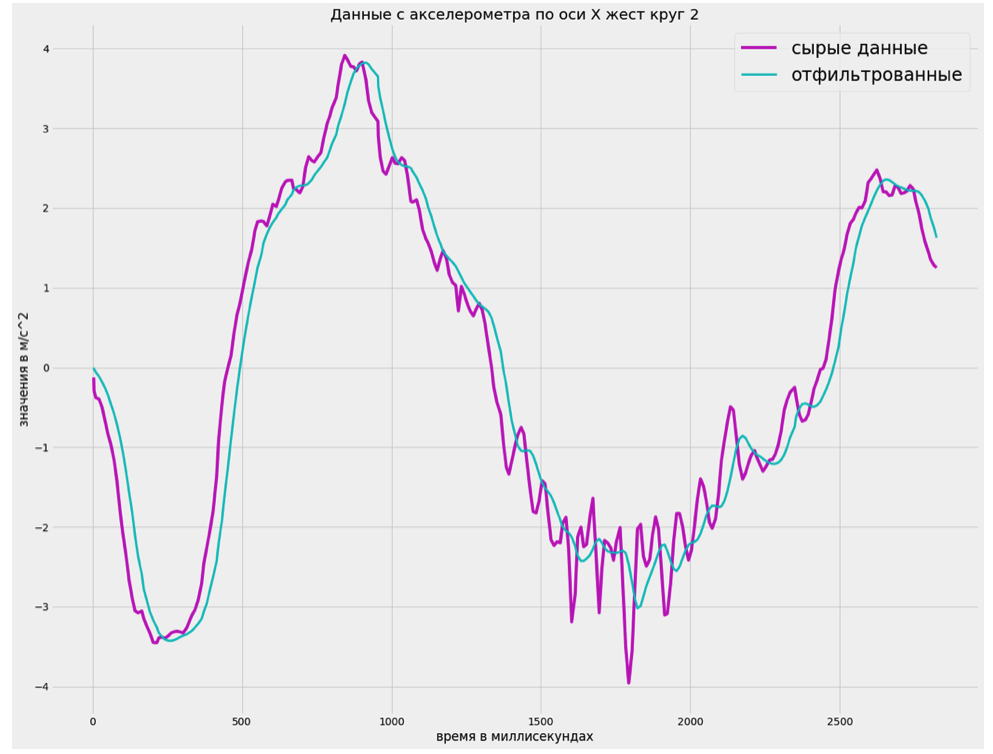
\includegraphics[width=0.75\textwidth]{farim/cirxres.png} & 
        \end{tabular}
    \end{center}
\end{figure}

\begin{figure}[H]
    \begin{center}
        \begin{tabular}{cc}
            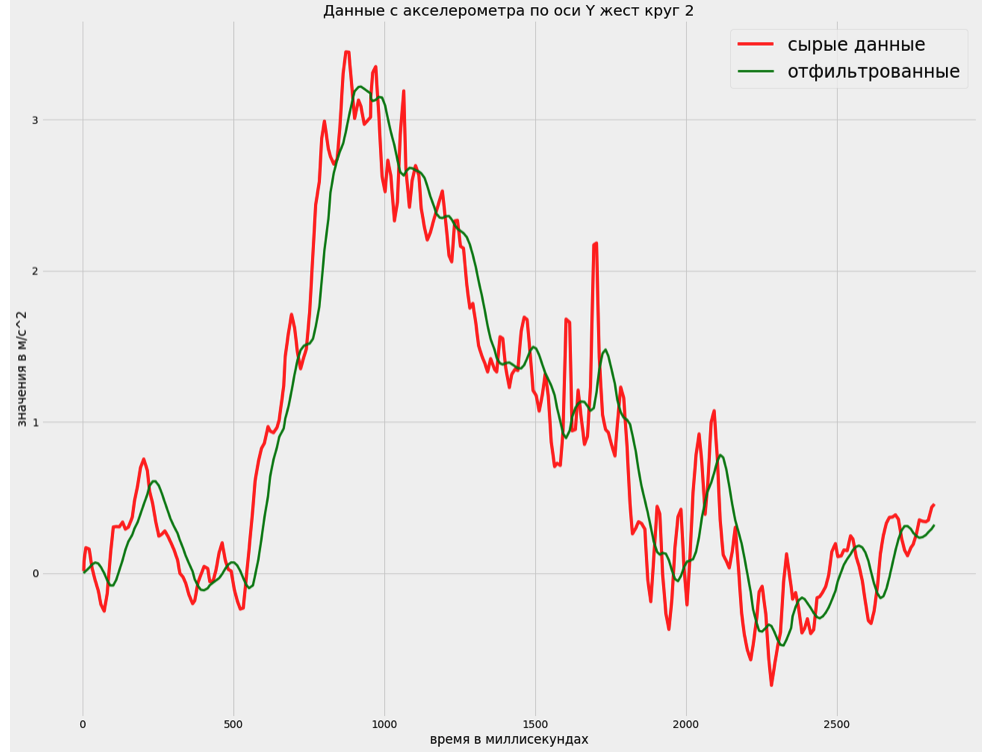
\includegraphics[width=0.75\textwidth]{farim/ciryres.png} & 
        \end{tabular}
    \end{center}
\end{figure}


\begin{figure}[H]
    \begin{center}
        \begin{tabular}{cc}
            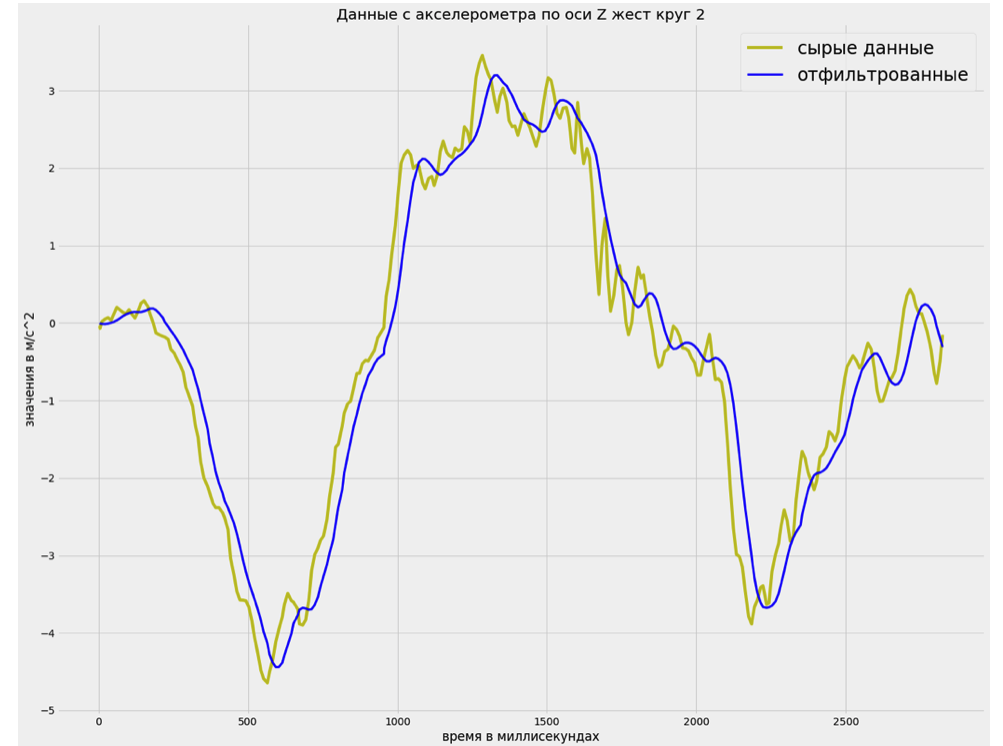
\includegraphics[width=0.75\textwidth]{farim/cirzres.png} & 
        \end{tabular}
    \end{center}
\end{figure}

\begin{figure}[H]
    \begin{center}
        \begin{tabular}{cc}
            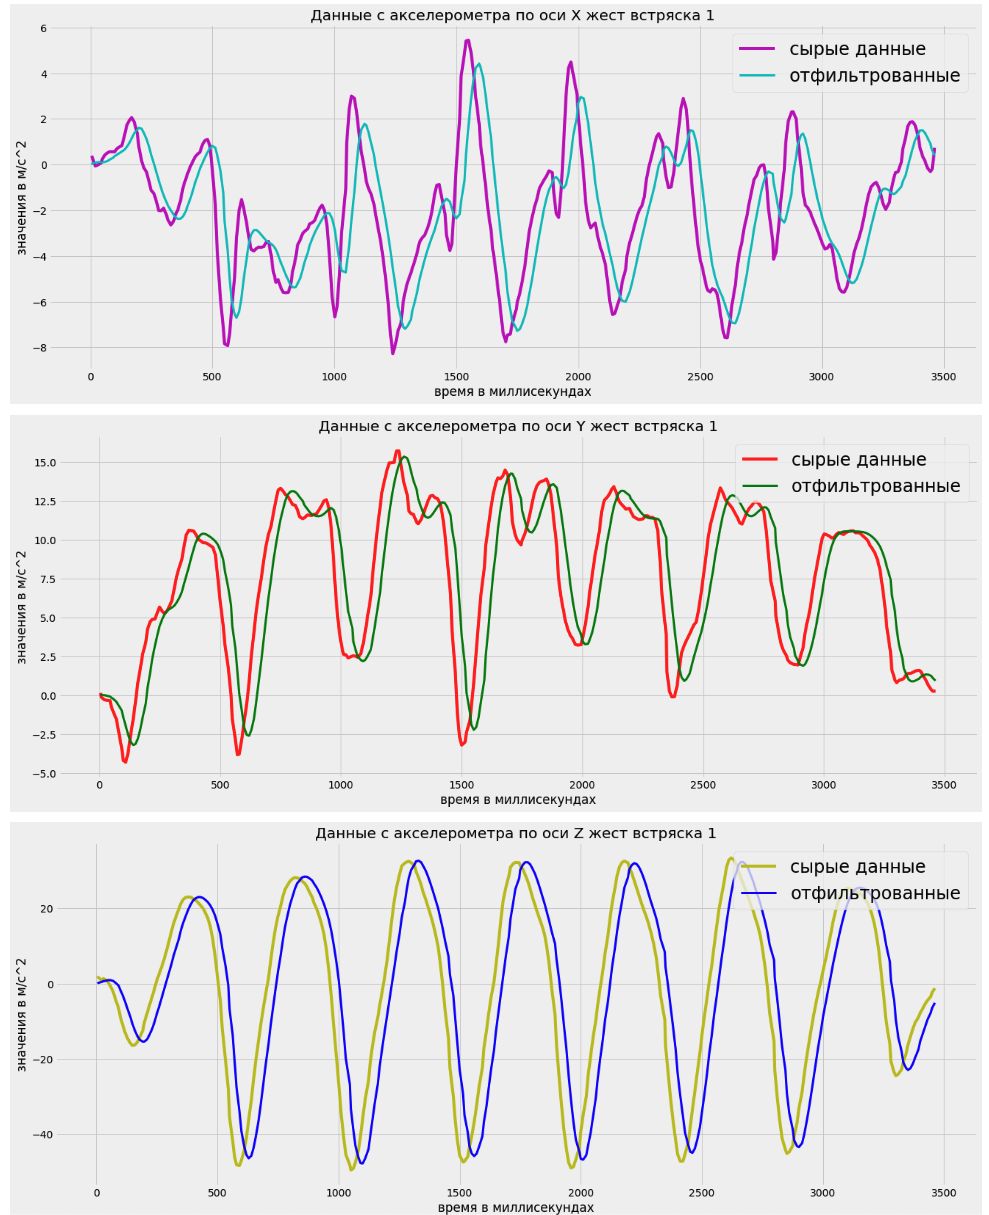
\includegraphics[width=1\textwidth]{farim/shak.png} & 
        \end{tabular}
    \end{center}
\end{figure}


\textbf{Итоги работы:} На графика хорошо видно, 
что фильтр справился со своей задачей. Мы получили более гладкий сигнал,
